\subsection{W-1 (AWD)}
Architektura databázového serveru, její podstatné komponenty a úloha databázového administrátora při jejich správě.

\subsubsection{Architektura databázového serveru}
Základním a výchozím procesem databázového serveru Postgresql je tzv. Postmaster. Je to hlavní démon který naslouchá na síťových portech a příjímá nová spojení od klientů. Každému nově příchozímu klientovi vytvoří nový proces - svůj fork, který s ním poté komunikuje, odbavuje dotazy a podobně. Díky odděleným procesům je zajištěna lepší bezpečnost a stabilita - když jeden proces spadne, ostatní pokračují v běhu. 

\begin{figure}[H]
    \centering
    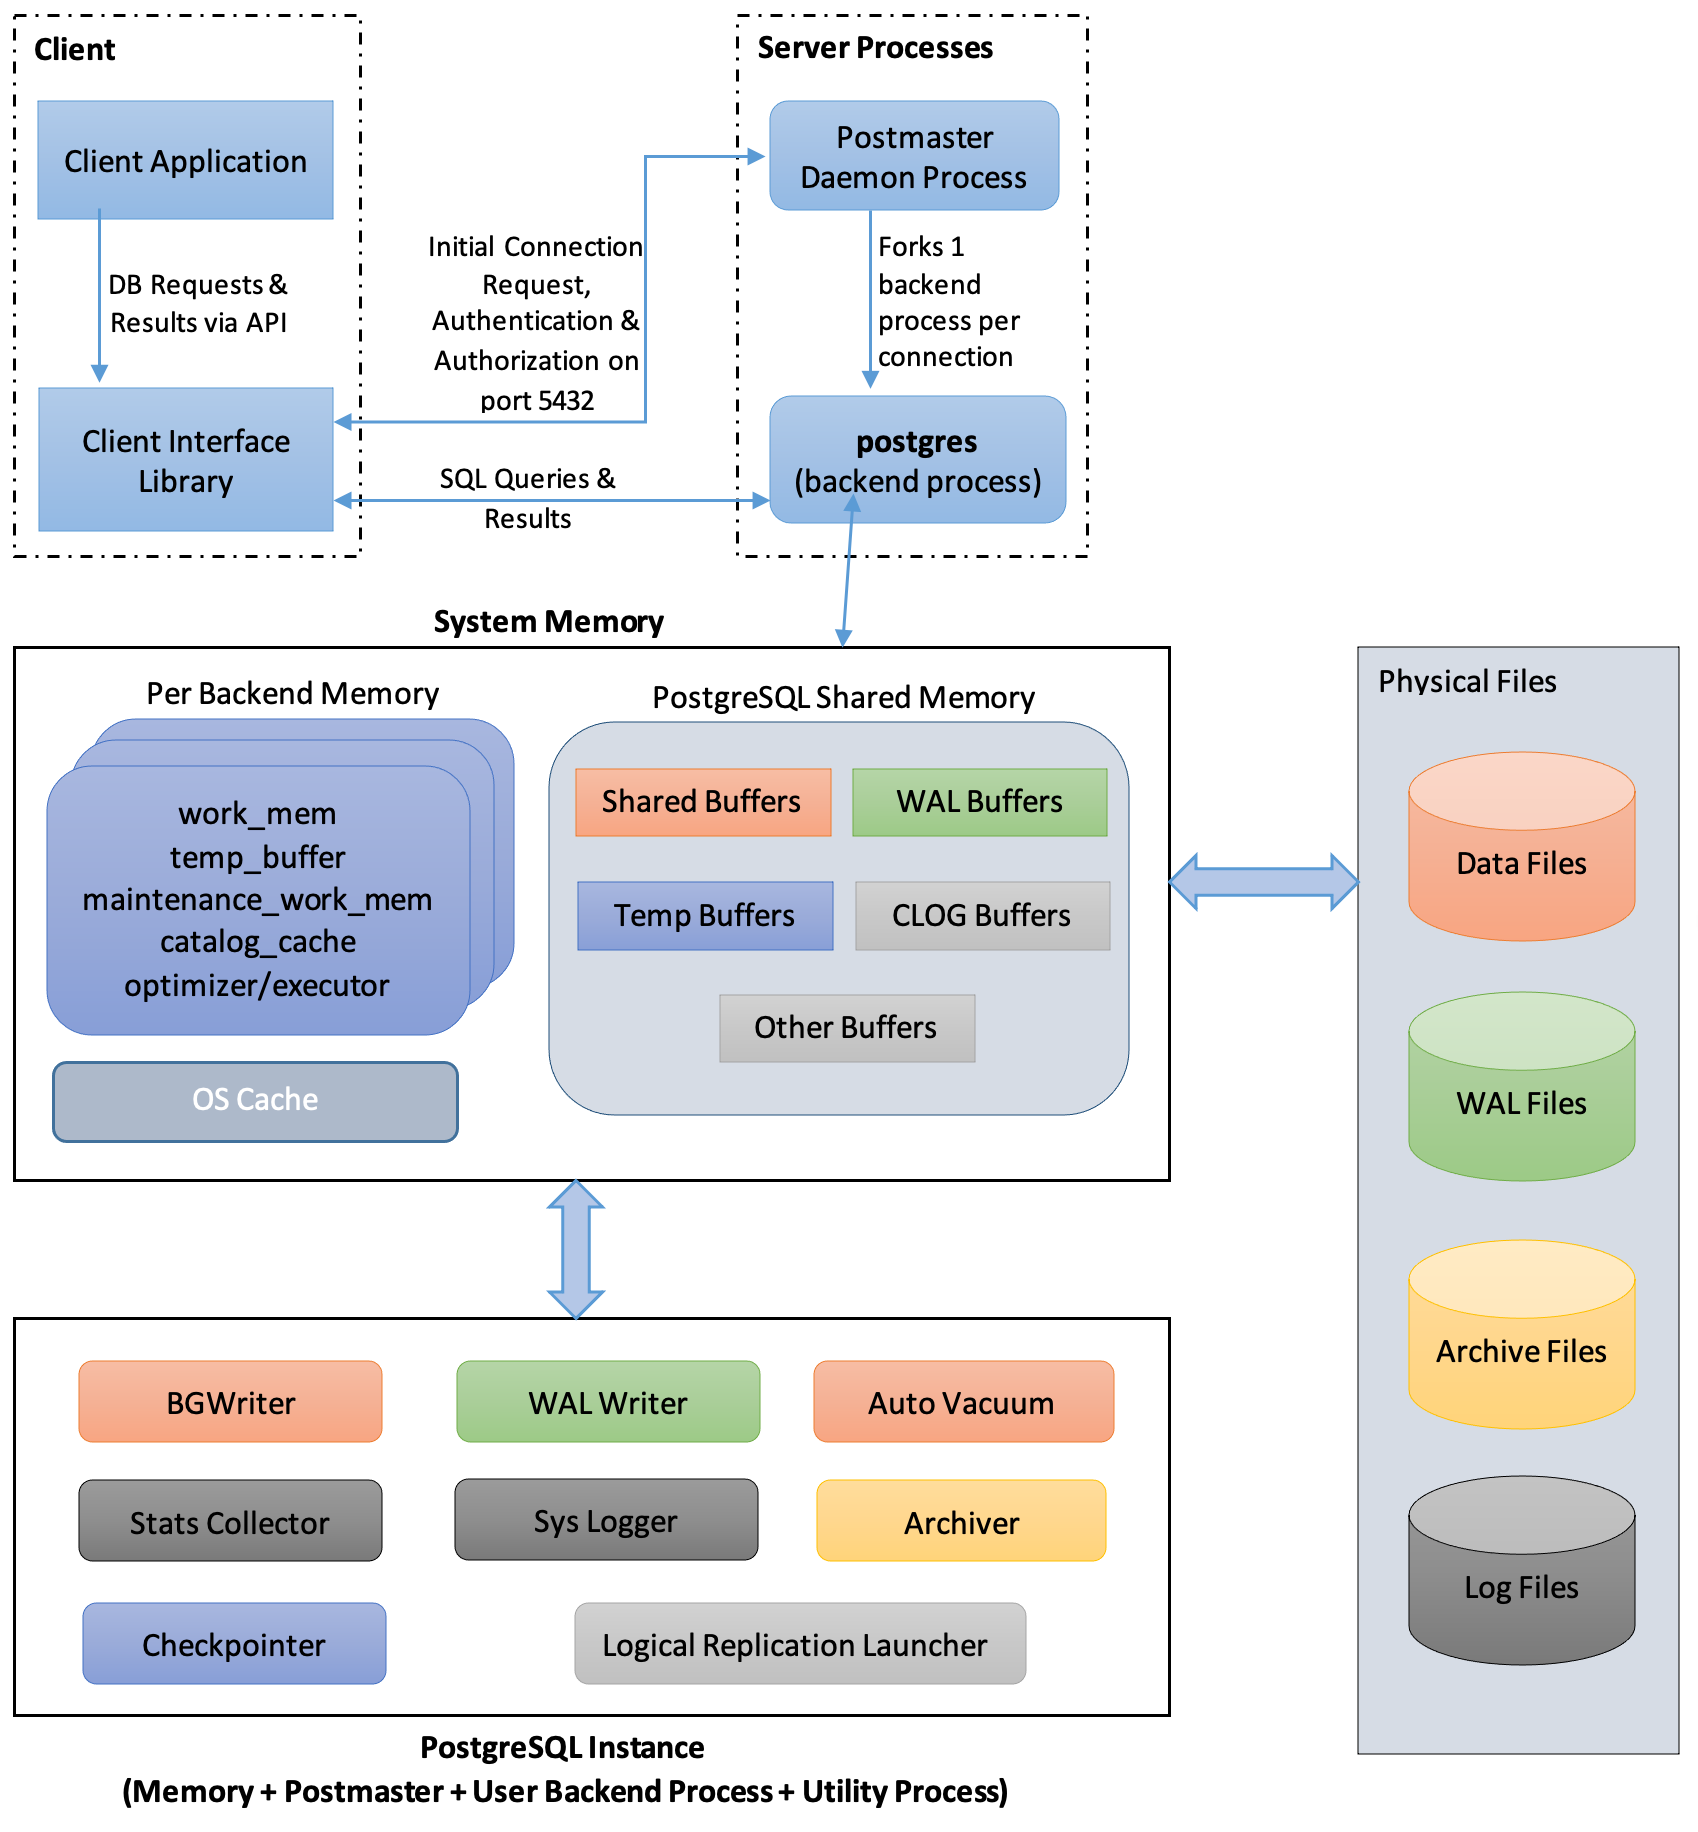
\includegraphics[width=0.75\textwidth]{img/postgresql_architecture.png}
    \caption{Architektura databázového serveru Postgresql}
\end{figure}

Databáze ještě obsahuje další podpůrné procesy:
\begin{itemize}
  \item Background writer - periodicky zapisuje změněné bloky z paměťového bufferu (shared buffer pool) na disk.
  \item WAL writer - zapisuje změny do WAL bufferu a periodicky je flushuje na disk. Je také důležitý pro zotavení aplikace po pádu a umožňuje point-in-time recovery.
  \item Checkpointer - vytváří tzv. checkpointy - body pro zotavení databáze. Checkpoint je snapshot, do kterého databázový server zapíše všechny změny v shared bufferu na disk a zároveň tento bod zapíše do WAL jako bod pro zotavení. Jinými slovy jedná se o snapshoter.
  \item Autovacuum Daemon - čistí tabulky od mrtvých řádků vzniklých během transakcí, automaticky spouští VACUUM a ANALYZE příkazy. Mrtvé řádky vznikají při UPDATE nebo DELETE operacích, kdy se stará verze řádku fyzicky nepřepíše, ale zůstává v tabulce jako mrtvý řádek. Toto je důsledek MVCC (Multi-Version Concurrency Control). VACUUM odstraňuje mrtvé řádky, ANALYZE aktualizuje statistiky a ještě se provádí Anti-wraparound VACUUM, který zabraňuje přetečení 32bitových identifikátorů transakce.
  \item Archiver - archivuje WAL soubory pro účely zálohování nebo replikace.
  \item Logical replication launcher - spouští procesy replikace pro logickou replikaci.
    \item Stats collector - shromažďuje statistiky o činnosti databáze a ukládá je do systémových tabulek. Tyto statistiky jsou užitečné pro ladění výkonu a monitorování databáze.
\end{itemize}

\subsubsection{Fyzické soubory}
Databáze využívá následující druhy fyzických souborů:
\begin{itemize}
    \item Data files - obsahují data tabulek a indexů. Každá tabulka a index je reprezentována jedním nebo více soubory na disku. Tyto soubory mají obvykle příponu .dat a jsou umístěny v adresáři pg\_data/base/\textit{oid\_db}/, kde oid\_db je identifikátor databáze.
  \item WAL soubory - obsahují záznamy o změnách provedených v databázi. Tyto soubory jsou důležité pro zotavení databáze po pádu.
  \item Konfigurační soubory - obsahují nastavení databázového serveru, jako je pg\_hba.conf (nastavení přístupu) a postgresql.conf (hlavní konfigurační soubor).
  \item Archive files - archivované WAL soubory, které jsou uloženy na jiném místě pro účely zálohování nebo replikace.
    \item Log files - obsahují záznamy o činnosti databázového serveru, jako jsou chybové hlášení, varování a informace o výkonu. Tyto soubory jsou užitečné pro ladění a monitorování databáze.
\end{itemize}

\subsection{Systémová paměť}
Databáze využívá následující druhy paměti:
\begin{itemize}
    \item Shared memory - sdílená paměť, která je používána všemi procesy databázového serveru. Obsahuje shared buffers, WAL buffers, Temp buffers, CLOG buffers (commit log) a další.
    \item Per backend memory - paměť, která je alokována pro každý proces databázového serveru. Obsahuje lokální proměnné, pracovní paměť a další dočasné struktury.
\end{itemize}

\subsubsection{Úloha databázového administrátora}
Databázový administrátor (DBA) je zodpovědný za správu databázového serveru a jeho komponentů. Mezi jeho hlavní úkoly patří:
\begin{itemize}
    \item instalace a konfigurace databázového serveru
    \item správa uživatelských účtů a oprávnění
    \item monitorování výkonu databáze a ladění výkonu
    \item zálohování a obnova databáze
    \item správa replikace a clusteringu
    \item správa bezpečnosti databáze
    \item správa aktualizací a patchů databázového serveru
\end{itemize}
